% AAMAS 2027 submission template (downloaded from the official conference
% endpoint on 2026-09-30).  Do not modify aamas.cls or its layout parameters.
\documentclass[sigconf,anonymous]{aamas}

\usepackage{booktabs}
\usepackage{graphicx}
\usepackage{microtype}
\usepackage{amsmath}
\usepackage{xspace}

\usepackage{balance}
% Unmodified copyright block supplied in the official AAMAS 2027 sample.
\makeatletter
\gdef\@copyrightpermission{
  \begin{minipage}{0.2\columnwidth}
   \href{https://creativecommons.org/licenses/by/4.0/}{
\includegraphics[width=0.90\textwidth]{by}}
  \end{minipage}\hfill
  \begin{minipage}{0.8\columnwidth}
   \href{https://creativecommons.org/licenses/by/4.0/}{This work is licensed under a Creative Commons Attribution International 4.0 License.}
  \end{minipage}
  \vspace{5pt}
}
\makeatother
\acmSubmissionID{TBD}
\submissionType{Research Paper Track}
\setcopyright{ifaamas}
\acmConference[AAMAS 2027]{Proc. of the 26th International Conference on
Autonomous Agents and Multiagent Systems (AAMAS 2027)}{3--7 May 2027}{Hanoi,
Vietnam}{M. Baldoni, F. Fang, W. Yeoh, N. Yorke-Smith (eds.)}
\copyrightyear{2027}
\acmYear{2027}
\acmDOI{}
\acmISBN{}

\newcommand{\vbe}{VBE\xspace}
\newcommand{\hh}{H--H\xspace}
\newcommand{\eh}{E$\rightarrow$H\xspace}
\newcommand{\mres}{MRES\xspace}

\title{Public Rules, Executed Behavior, and Welfare in a Language-Model Economy}

\author{Anonymous Authors}
\affiliation{\institution{Anonymous Institution}}

\ccsdesc[500]{Computing methodologies~Multi-agent systems}
\ccsdesc[300]{Computing methodologies~Agent / discrete models}
\ccsdesc[300]{Computing methodologies~Natural language processing}


\begin{document}

\begin{abstract}
Public natural-language rules for language-model agents are usually judged by
whether agents perform the action the rule names.  We test that practice in the
Verification Budget Economy, an eight-agent random-matching economy with scarce
verification checks.  A public announcement naming Easy-to-Hard gifts raises
welfare by 2.06 points per account over a no-recommendation announcement
(14/14 paired seeds), yet an exact accounting identity attributes the gain to
Hard--Hard check swaps---mutual cooperation in an unnamed stage game that is a
Prisoner's Dilemma---net of dominated Hard-to-Easy giving the same text induces.
Under a byte-identical gift announcement, blocking Hard--Hard transfers after the
model responds lowers welfare by 3.21 (12/12 seeds).  Replaying the frozen
traces through the engine, we compare first decisions at states that are
byte-identical except for the announcement: the named gift is engaged but
collapses after one meeting, whereas cross-role Hard--Hard giving is raised
directly by the text, including by a harmful Easy--Easy directive obeyed in 113
of 114 meetings.  Explicit exclusion clauses bound the response; positive role
predicates do not.
\end{abstract}

\keywords{language-model agents, multi-agent systems, public rules, norms,
causal mechanisms, welfare, agent-based simulation}

\maketitle

\section{Introduction}

Teams, markets, and simulations of language-model agents increasingly
coordinate through public rules written in natural language.  The usual check of such a rule
is whether agents perform the action it names and whether an aggregate outcome
improves.  That check conflates four objects: the proposals agents make, the
transactions the environment executes from pairs of proposals, the state those
transactions produce, and the welfare that results.  A rule can be followed in
its named relation and still owe its effect to a relation it never mentions.

We study this gap in the Verification Budget Economy (\vbe), where Hard agents
need verification checks, Easy agents have spare ones, and the engine executes
only compatible pairs of proposals.  Three prospectively frozen studies with a
hosted model supply the causal comparisons; a zero-call reanalysis of their
frozen traces supplies the accounting and the fixed-state comparisons.  The
results form one chain:

\begin{itemize}
\item \emph{Welfare comes from an unnamed relation.}  The engine implies that a
Hard--Hard meeting is a strict Prisoner's Dilemma and that giving in an
Easy--Hard meeting is individually dominated for both roles.  A gift
announcement naming Easy-to-Hard gifts raises welfare, and an exact accounting
identity attributes the gain to Hard--Hard swaps net of wasteful Hard-to-Easy
gifts.  Blocking Hard--Hard transfers under the identical announcement removes
the gain (\S\ref{sec:welfare}).
\item \emph{The text acts on unnamed roles directly.}  Because each prompt is a
function of reconstructable state, we can find first decisions taken from states
that are byte-identical across arms except for the announcement.  There, the
named Easy-to-Hard gift is engaged, and Hard--Hard giving is raised by the gift
text and by a harmful Easy--Easy directive.  Explicit exclusion clauses bound
the response; positive role predicates do not (\S\ref{sec:fixed}).
\item \emph{Closed-loop dynamics separate the two.}  The named gift collapses
after an Easy agent's first meeting, whereas Hard--Hard cooperation and harmful
Easy--Easy compliance persist for the whole run (\S\ref{sec:dynamics}).
\end{itemize}

The contribution is an identification design and the result it produces, not a
reminder that intention differs from execution.  Execution-layer intervention
under a fixed prompt, exact transaction accounting, fixed-state comparison from
frozen logs, and an engaged harmful control together rule out the intuitive
explanation---that the rule works because agents do what it says---and locate
both the welfare channel and the failure modes.  The claim concerns a hosted
model population in one economy, not private belief, common knowledge, or a
self-enforcing institution.

\section{Environment}
\label{sec:env}

\subsection{Rules and state}

\vbe has $n=8$ persistent accounts and $T=24$ rounds; the supplement lists every
parameter.  All accounts start with score 0, and
four random accounts start with one \emph{mark} each.  Marks have no direct or
terminal value and persist across rounds.  Each round proceeds as follows.

\begin{enumerate}
\item \emph{Roles and endowments.}  Exactly four accounts are drawn Hard and four
Easy.  Every account receives $B=1$ check.  An Easy account is paid $R=3$
immediately.
\item \emph{Matching.}  Accounts are shuffled into four pairs, and each pair meets
independently with probability $q=0.4$, so an account has at most one meeting per
round and roles are independent of pairing.
\item \emph{Proposals.}  Each party to a meeting simultaneously proposes
\texttt{giveCheck}, \texttt{giveChits} (0 or 1 marks), and \texttt{requireChit}.
\item \emph{Resolution.}  In priority order: if both give and neither requires a
mark, the checks are \emph{swapped}; if one gives while requiring a mark and the
other offers one, a \emph{sale} executes; if one gives without requiring a mark,
it is a one-way \emph{gift}; otherwise nothing moves.  A received check is a
verification source; it is not added to the recipient's inventory.
\item \emph{Settlement.}  A Hard account that received a check uses it and
succeeds with probability $p_P=0.93$; otherwise it uses its own check and
succeeds with probability $p_H=0.32$.  Success pays $R$.  Every check still in
inventory pays $v=0.5$, and checks expire.
\end{enumerate}

Scores, marks, and each account's last $K=4$ meetings persist.  The prompt shows
the round, the agent's role, checks, marks, and score, the partner's role,
checks, and marks, and the agent's own last four meetings; it never shows the
partner's score or history.  One payoff draw per account per round is
pre-generated from the seed, so arms sharing a seed share roles, pairings, and
payoff draws.

\subsection{Transaction payoffs and stage games}
\label{sec:payoffs}

\begin{table}[t]
\caption{Expected direct payoff change of one executed transfer relative to no
transfer, derived from the engine.  A sale moves the same payoffs as a gift in
the same direction because marks are valueless.}
\label{tab:payoffs}
\small
\centering
\begin{tabular}{@{}lrrr@{}}
\toprule
Executed transfer & Giver & Receiver & Total \\
\midrule
H--H swap & $+1.83$ & $+1.83$ & $+3.66$ \\
E--H swap (E is ``giver'') & $-0.50$ & $+1.83$ & $+1.33$ \\
E--E swap & $-0.50$ & $-0.50$ & $-1.00$ \\
One-way E$\rightarrow$H & $-0.50$ & $+2.33$ & $+1.83$ \\
One-way H$\rightarrow$H & $-0.96$ & $+2.33$ & $+1.37$ \\
One-way H$\rightarrow$E & $-0.96$ & $0.00$ & $-0.96$ \\
One-way E$\rightarrow$E & $-0.50$ & $0.00$ & $-0.50$ \\
\bottomrule
\end{tabular}
\end{table}

Table~\ref{tab:payoffs} lists the expected change for every transfer the engine
can execute.  Each entry is checked against the engine by integrating its
settlement over the payoff-draw strata, and an exhaustive test covers all 4,096
local meeting states (\S\ref{sec:audit}).  Two rows matter most.  An E--H
\emph{swap} is worth $1.33$, not $1.83$: the Hard agent gives away a check it
would otherwise salvage, and the Easy agent cannot use the check it receives.  A
one-way H$\rightarrow$E gift destroys $0.96$.

\begin{table}[t]
\caption{Expected round payoffs (row, column) in a Hard--Hard meeting implied by
Table~\ref{tab:payoffs}.  Keeping is strictly dominant and mutual giving maximizes
welfare: a strict Prisoner's Dilemma.}
\label{tab:pd}
\small
\centering
\begin{tabular}{@{}lcc@{}}
\toprule
& Partner keeps & Partner gives \\
\midrule
Keep & $(0.96,\ 0.96)$ & $(3.29,\ 0.00)$ \\
Give & $(0.00,\ 3.29)$ & $(2.79,\ 2.79)$ \\
\bottomrule
\end{tabular}
\end{table}

The identities imply the stage games.  An H--H meeting is a strict Prisoner's
Dilemma (Table~\ref{tab:pd}): keeping is dominant, and mutual giving maximizes
welfare.  In an E--H meeting, keeping is
strictly dominant for both roles, and the welfare-maximizing outcome is a one-way
E$\rightarrow$H gift, which costs the Easy agent $0.5$.  Every welfare-improving
transfer therefore requires an agent to give up private payoff.  The population
game is repeated under random rematching with private four-meeting histories,
where cooperation can in principle be sustained by community
enforcement~\cite{kandori1992,ellison1994}; our design does not identify such a
mechanism.

Two model-free benchmarks run on the same seeds, schedules, and draws.  The
\emph{ex-ante first best} maximizes expected welfare meeting by meeting over the
engine's action space without using realized draws: an H--H swap, a one-way
E$\rightarrow$H gift, and no transfer otherwise.  It is a planner benchmark, not
an equilibrium.  The \emph{ex-post first best} uses realized draws and bounds
attainable welfare.  \emph{Never-transfer} sets the baseline.

\section{Studies and Inference}
\label{sec:design}

All model studies use \texttt{deepseek-flash} in one provider-labeled serving era
at temperature zero.  Every protocol, seed list, prompt, contrast, and gate was
hash-frozen locally before its first target call; none was externally
registered.  Each study is bracketed by a 14-call provider-health check before
the first and after the last target call, with external controls, dominance
anchors, entropy, returned-model, catalog, and fingerprint gates; all brackets
reported here are healthy and identity-consistent.  The supplement records the
anomalous earlier service window that motivated the bracket.

\paragraph{W-CO (discovery).}  Gift versus money announcements on 18 fresh
paired seeds.  Its welfare contrast was prospective; its planned
gift-for-sale substitution gate failed, and the H--H channel was found
afterwards.  We use it only as discovery and as a third replication of the
fixed-state results.

\paragraph{W-RG (execution intervention).}  Four arms on 12 fresh paired
seeds: neutral; gift; gift with H--H check giving blocked; gift with
unconditional E$\rightarrow$H give proposals blocked.  The three gift arms show
the model the same announcement.  After the model responds, a filter sets only
\texttt{giveCheck} to false on eligible proposals and leaves the other fields
unchanged; the engine then executes as usual and later prompts reflect the
changed history.  W-RG estimates the dynamic total effect of changing the
execution contract under a fixed announcement.

\paragraph{W-SGB (package boundary).}  Seven announcements on 14 fresh paired
seeds under unmodified execution (Table~\ref{tab:arms}).  The harmful E--E
directive names a transfer that destroys $1.0$ per execution and carries its
own frozen engagement gate.  Packages other than the three historical anchors
are not length-matched, so contrasts identify whole packages.

\begin{table*}[t]
\caption{W-SGB announcement packages.  Every package also states that it is a
public statement rather than an engine rule, may be followed or ignored, and that
agents should maximize their own score.  The supplement reproduces every package
verbatim.}
\label{tab:arms}
\footnotesize
\centering
\begin{tabular}{@{}lp{0.47\textwidth}l@{}}
\toprule
Arm & Distinguishing clause (abridged) & Named relation; explicit exclusion \\
\midrule
Neutral & ``announces no exchange recommendation'' & none \\
Gift exact & ``an Easy agent gives a leftover check to a Hard agent'' & E $\rightarrow$ H gift \\
Easy only & ``only an Easy agent gives \ldots{} A Hard agent does not give'' & E $\rightarrow$ H gift; excludes Hard actors \\
Any holder & ``any agent who holds a leftover check gives it to a Hard agent'' & \{E,H\} $\rightarrow$ H gift \\
Hard partner & ``an agent gives \ldots{} only when the current partner is Hard \ldots{} do not give \ldots{} when the current partner is Easy'' & \{E,H\} $\rightarrow$ H gift; excludes Easy partners \\
Money exact & ``a mark is accepted as payment \ldots{} a Hard agent who holds a mark may buy'' & E $\rightarrow$ H sale \\
Harmful E--E & ``when two Easy agents meet \ldots{} each gives that check to the other'' & E $\leftrightarrow$ E swap \\
\bottomrule
\end{tabular}
\end{table*}

\paragraph{Inference.}  Let $Y_s(d,e)$ be the seed-$s$ population outcome under
announcement $d$ and execution contract $e$; the seed fixes initial state,
roles, pairings, and payoff draws.  W-RG and W-SGB estimate, respectively,
\begin{align*}
\tau_{\mathrm{RG}}&=\tfrac{1}{12}\textstyle\sum_s\bigl[Y_s(d_{\mathrm{gift}},e_{\mathrm{std}})-Y_s(d_{\mathrm{gift}},e_{\neg\mathrm{HH}})\bigr],\\
\tau_{\mathrm{SGB}}&=\tfrac{1}{14}\textstyle\sum_s\bigl[Y_s(d_1,e_{\mathrm{std}})-Y_s(d_0,e_{\mathrm{std}})\bigr].
\end{align*}
Both include downstream feedback through holdings and histories, so the
inferential unit is the paired seed-level trajectory, not a meeting or account,
and neither identifies a natural indirect effect~\cite{hudgens2008,aronow2017}.
We report percentile bootstrap intervals (20,000 resamples of seed differences;
pointwise, not simultaneous) and one-sided exact sign-flip $p$-values for
$\Delta>0$ under a zero-centered sign-symmetry null.  W-SGB applies Holm
correction at $0.025$ within its eight H--H and eight welfare contrasts.  A
frozen gate passes when the mean reaches the minimum relevant effect size
(\mres: $0.25$ for swap rate, $0.5$ for welfare) and the adjusted $p\le0.025$.
Passing a gate shows a large estimate and a nonzero effect; it does not show
$\Delta>\mres$.  We therefore add supplementary exact tests of
$H_0{:}\,\Delta\le\mres$ and leave-one-seed-out ranges.  With 12 or 14 seeds the
smallest attainable one-sided $p$ is $2^{-12}$ or $2^{-14}$, reached whenever
every seed agrees in sign, so we report sign counts throughout.

\subsection{Zero-call reanalysis of frozen traces}
\label{sec:audit}

The reanalysis adds no model call and changes no frozen artifact.  We replay
every frozen run through the frozen engine by feeding back its recorded
proposals.  Because roles, pairings, and draws come from the seed alone, the
replay reproduces all 182 runs exactly (every final score and every meeting
resolution), recovering the exact prompt behind each of the 14,010 decisions, a
count equal to the three studies' frozen call totals.  This supports three
analyses.  \emph{Accounting:} each run's welfare equals its never-transfer
welfare plus the realized contribution of each executed transfer, computed from
the regenerated payoff draws; the identity holds exactly in all 182 runs.
\emph{Fixed states:} at an agent's first meeting, its prompt carries no
treatment-dependent history, and the reconstructed prompts are byte-identical
across arms once the announcement is removed (verified for every first
meeting); comparing arms there isolates the announcement's effect on that
decision.  \emph{Engine validation:} an exhaustive test enumerates every role
pair, inventory, and proposal combination (4,096 cases) and checks resource
conservation, the filters, and settlement against Table~\ref{tab:payoffs}.
These analyses are post hoc and descriptive with respect to the frozen studies.

\section{Results}

\subsection{Welfare comes from an unnamed cooperation channel}
\label{sec:welfare}

The gift announcement raises welfare.  In W-SGB it exceeds neutral by
$2.0625$ points per account ($[1.429,2.813]$, 14/14 seeds), raising the H--H
swap rate by $0.607$; W-CO's gift-minus-money contrast ($+2.333$, 17/18 seeds)
and W-RG's gift-minus-neutral contrast ($+1.682$, 9/12 seeds) agree in sign
(Table~\ref{tab:contrasts}).

\begin{figure*}[t]
  \centering
  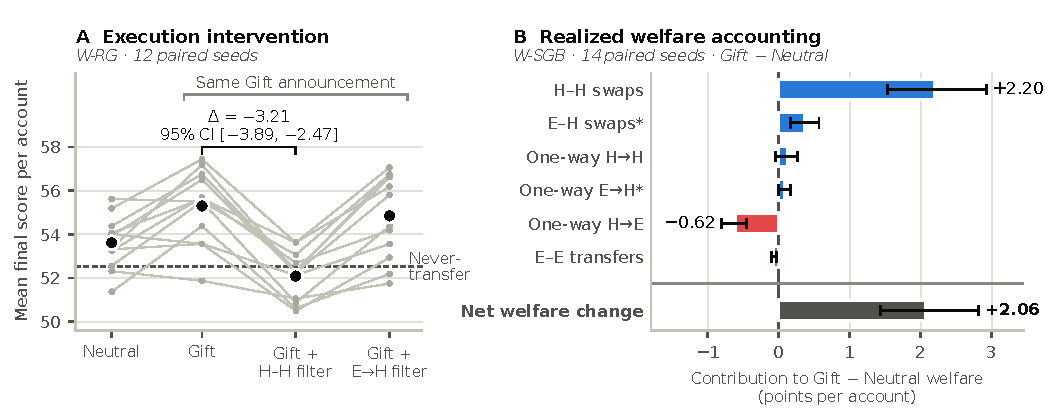
\includegraphics[width=0.98\textwidth]{figures/VBE-x1-fig-mechanism.pdf}
  \Description{Left: seed-level welfare for twelve W-RG seeds across four arms,
  with arm means and dashed never-transfer and ex-ante first-best lines; welfare
  drops from about 55.3 under gift to about 52.1 when Hard--Hard transfers are
  blocked, near the never-transfer line.  Right: horizontal bars decomposing the
  W-SGB gift-minus-neutral welfare difference by transfer type: Hard--Hard swaps
  +2.20, Easy--Hard swaps +0.36, one-way Hard-to-Hard +0.12, one-way
  Easy-to-Hard +0.08, one-way Hard-to-Easy -0.62, Easy--Easy -0.07, net +2.06,
  with W-RG values as hollow diamonds.}
  \caption{(A) W-RG: seed-level welfare (lines connect a seed's four paired runs).
  Blocking H--H transfers under the identical gift announcement removes the gift's
  gain.  Dashed lines are model-free benchmarks on the same seeds.  (B) Exact
  accounting of the gift-minus-neutral welfare difference by executed transfer type
  (W-SGB bars; W-RG diamonds).  This is an accounting identity, not a mediation
  estimate: arms differ in which transfers occur.}
  \label{fig:mechanism}
\end{figure*}

\paragraph{Where the gain comes from.}  The named transfer is almost absent from
the realized trace.  In W-SGB's gift arm, 105 of 125 H--H meetings end in swaps
(27 under neutral), while only 9 of 304 E--H meetings end in a one-way
E$\rightarrow$H gift.  Figure~\ref{fig:mechanism}B decomposes the welfare
difference exactly: H--H swaps contribute $+2.20$ per account and E--H swaps
$+0.36$, while 99 one-way H$\rightarrow$E gifts (3 under neutral) cost $0.62$.
W-RG gives the same pattern ($+2.41$ from H--H swaps, $-1.13$ from
H$\rightarrow$E gifts).  The announcement therefore buys welfare through
cooperation in the unnamed Prisoner's Dilemma and pays for part of it with a
dominated, welfare-destroying transfer the same text induces.  Reciprocity also
costs welfare in the named relation: in W-RG's gift arm, 25 of 26 feasible
E$\rightarrow$H gift intentions met an unconditional Hard give and resolved as
E--H swaps, each worth $0.5$ less than the one-way gift (12.5 points in total).
Joint proposals show where these transfers come from: in the gift arm's E--H
meetings, only the Easy agent gave in 9, only the Hard agent in 99, both in 28,
and neither in 168.  Table~\ref{tab:welfare} places every package against
model-free benchmarks on the same seeds.  The gift package captures 35\% of the
ex-ante feasible gain; the Hard-partner package captures the most, 38\%, because
it keeps H--H swaps (115) while nearly eliminating H$\rightarrow$E gifts (18).
Mutual H--H giving is not simply two independent proposals: under neutral it
occurs in 27 of 125 meetings, against about 8 expected from the marginal give
rate, whereas under gift it matches independence (105 versus 104).

\begin{table*}[t]
\caption{Absolute welfare and executed transfers by W-SGB package (14 seeds,
same schedules and payoff draws).  Gain is welfare minus the never-transfer
benchmark; share is gain divided by the ex-ante first best's gain.  Transfer
columns count executed meetings out of 125 H--H, 304 E--H, and 114 E--E meetings
per arm.}
\label{tab:welfare}
\footnotesize
\centering
\begin{tabular}{@{}lrrrrrrrr@{}}
\toprule
Package or benchmark & Welfare & Gain & Share & H--H swaps & E--H swaps & One-way E$\rightarrow$H & One-way H$\rightarrow$E & E--E swaps \\
\midrule
Neutral & 55.28 & 1.04 & 0.12 & 27 & 0 & 0 & 3 & 0 \\
Gift exact & 57.34 & 3.10 & 0.35 & 105 & 28 & 9 & 99 & 2 \\
Easy only & 55.23 & 0.99 & 0.11 & 29 & 0 & 0 & 16 & 1 \\
Any holder & 57.25 & 3.00 & 0.34 & 111 & 28 & 7 & 95 & 0 \\
Hard partner & 57.68 & 3.44 & 0.38 & 115 & 1 & 4 & 18 & 0 \\
Money exact & 55.07 & 0.83 & 0.09 & 21 & 0 & 0 & 0 & 0 \\
Harmful E--E & 55.46 & 1.22 & 0.14 & 75 & 1 & 3 & 35 & 113 \\
\midrule
Never transfer & 54.24 & 0 & 0 & 0 & 0 & 0 & 0 & 0 \\
Always give & 60.81 & 6.57 & 0.73 & 125 & 304 & 0 & 0 & 114 \\
Ex-ante first best & 63.19 & 8.95 & 1 & 125 & 0 & 304 & 0 & 0 \\
Ex-post first best (uses realized draws) & 63.26 & 9.02 & 1.01 & --- & --- & --- & --- & --- \\
\bottomrule
\end{tabular}
\end{table*}

\paragraph{Execution intervention.}  W-RG holds the announcement fixed and
removes the H--H channel after the model responds.  Welfare falls by $3.208$
($[2.469,3.891]$, 12/12 seeds, Figure~\ref{fig:mechanism}A), from $55.30$ to
$52.09$---below the same seeds' never-transfer benchmark ($52.53$) in 10 of 12
seeds.  Without H--H circulation, the remaining transfers induced by the gift
announcement are net negative.  Removing transfers worth $3.66$ each will lower
welfare; the result is informative because the removed channel is the one the
announcement does not name, and because what remains of the announcement's
effect is wasteful.  The E$\rightarrow$H filter changed little: of its 20
blocked proposals, 16 would have produced E--H swaps and instead executed as
one-way H$\rightarrow$E gifts, and 4 would have produced one-way E$\rightarrow$H
gifts.  The regime contrast ``E$\rightarrow$H-blocked minus H--H-blocked''
($+2.760$, 12/12) therefore compares keeping H--H circulation with keeping the
little that the E$\rightarrow$H path carried.

W-RG has no neutral-with-H--H-blocked arm, so it does not identify how much of
the gift-versus-neutral effect depends on the H--H path; the accounting
identity above is consistent with nearly all of it but is not a causal
decomposition.  The supplement gives a frozen-ready protocol for the
announcement-by-execution factorial that would.

\begin{table*}[t]
\caption{Prospective paired contrasts.  CIs are pointwise percentile bootstrap
intervals over seeds; $+/-/0$ counts seeds by sign.  $p$ is the one-sided exact
sign-flip $p$ for $\Delta>0$, Holm-adjusted within each W-SGB endpoint family.
$p_{\mres}$ tests $H_0{:}\,\Delta\le\mres$ (supplementary; Holm within each W-SGB
family).  Frozen gates require mean $\ge\mres$ and $p\le0.025$.}
\label{tab:contrasts}
\footnotesize
\centering
\setlength{\tabcolsep}{4pt}
\begin{tabular}{@{}lrrcrrl@{}}
\toprule
W-RG (12 seeds) & $\Delta$ & 95\% CI & $+/-/0$ & $p$ & $p_{\mres}$ & Gate \\
\midrule
Gift $-$ neutral, welfare & 1.682 & [0.854, 2.463] & 9/3/0 & .0034 & .011 & pass \\
Gift $-$ H--H-blocked, welfare & 3.208 & [2.469, 3.891] & 12/0/0 & .00024 & .00024 & pass \\
E$\rightarrow$H-blocked $-$ H--H-blocked, welfare & 2.760 & [2.094, 3.412] & 12/0/0 & .00024 & .00024 & pass \\
Gift $-$ H--H-blocked, H--H swap rate & 0.753 & [0.633, 0.862] & 12/0/0 & .00024 & .0020 & pass \\
\bottomrule
\end{tabular}

\vspace{6pt}
\begin{tabular}{@{}lrrcrrrrcrr@{}}
\toprule
& \multicolumn{5}{c}{H--H swap rate (\mres{} 0.25)} & \multicolumn{5}{c}{Welfare (\mres{} 0.5)} \\
\cmidrule(lr){2-6}\cmidrule(l){7-11}
W-SGB (14 seeds) & $\Delta$ & 95\% CI & $+/-/0$ & $p$ & $p_{\mres}$ & $\Delta$ & 95\% CI & $+/-/0$ & $p$ & $p_{\mres}$ \\
\midrule
Gift $-$ neutral & .607 & [.510, .714] & 14/0/0 & .00049 & .00049 & 2.063 & [1.429, 2.813] & 14/0/0 & .00049 & .00085 \\
Gift $-$ money & .663 & [.568, .755] & 14/0/0 & .00049 & .00049 & 2.268 & [1.670, 2.960] & 14/0/0 & .00049 & .00049 \\
Gift $-$ harmful E--E & .229$^\dagger$ & [.105, .351] & 10/3/1 & .0054 & 1.0 & 1.875 & [1.348, 2.433] & 14/0/0 & .00049 & .0011 \\
Harmful E--E $-$ neutral & .378 & [.287, .474] & 14/0/0 & .00049 & .027 & .188 & [$-$.339, .710] & 9/5/0 & .51 & 1.0 \\
Gift $-$ Easy only & .592 & [.482, .697] & 14/0/0 & .00049 & .00049 & 2.112 & [1.464, 2.813] & 14/0/0 & .00049 & .0011 \\
Any holder $-$ neutral & .658 & [.549, .771] & 14/0/0 & .00049 & .00049 & 1.969 & [1.295, 2.696] & 14/0/0 & .00049 & .0011 \\
Hard partner $-$ neutral & .703 & [.596, .810] & 14/0/0 & .00049 & .00049 & 2.406 & [1.759, 3.107] & 14/0/0 & .00049 & .0011 \\
Money $-$ neutral & $-$.056 & [$-$.126, $-$.001] & 1/5/8 & .97 & 1.0 & $-$.205 & [$-$.339, $-$.071] & 1/9/4 & .996 & 1.0 \\
\bottomrule
\multicolumn{11}{l}{$^\dagger$Significant but below the 0.25 \mres, so its frozen gate fails.  Every other row with mean $\ge\mres$ and $p\le0.025$ passes its frozen gate.}
\end{tabular}
\end{table*}

The stricter supplementary test confirms every passing frozen gate, with one
exception: the harmful directive's H--H effect rejects $\Delta\le0.25$ before
correction ($p=0.0089$) but not after Holm ($0.027$).  Every passing contrast
keeps its mean above \mres{} when any single seed is dropped.

\subsection{The text acts on unnamed roles directly}
\label{sec:fixed}

Aggregate role-conditional proposal rates mix two sources: the announcement
changes what an agent does in a given state, and it changes which states agents
reach.  First decisions remove the second source.  Figure~\ref{fig:scope}A
shows, for every W-SGB package, the unconditional-give rate at each agent's first
meeting, where the prompt differs across arms only in the announcement (18
H$\rightarrow$H, 35 H$\rightarrow$E, 39 E$\rightarrow$H, and 20 E$\rightarrow$E
decisions per arm).

\begin{figure*}[t]
  \centering
  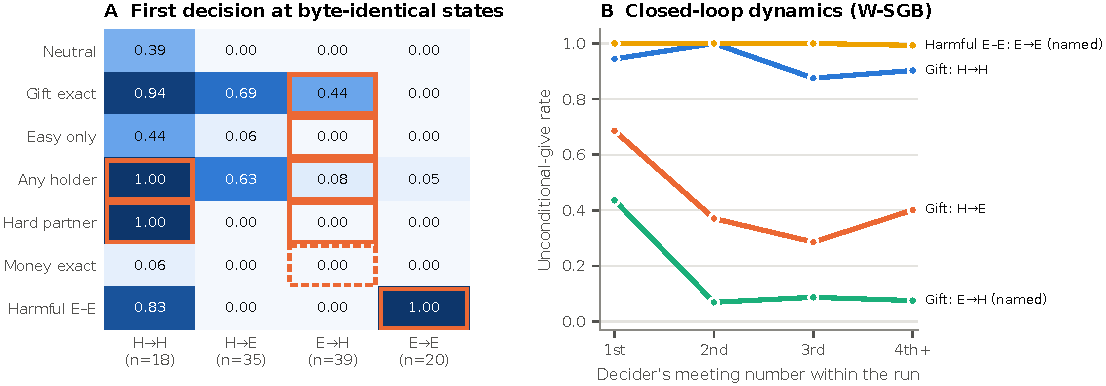
\includegraphics[width=0.98\textwidth]{figures/VBE-x1-fig-scope.pdf}
  \Description{Left: a heatmap with seven announcement packages as rows and four
  directed role cells as columns, showing the first-decision give rate; orange
  outlines mark the cells each package names.  Gift exact gives 0.94 to Hard
  partners when Hard, 0.69 from Hard to Easy, and 0.44 from Easy to Hard; the
  harmful Easy--Easy directive gives 1.00 in its named cell and 0.83 Hard to
  Hard; neutral gives 0.39 Hard to Hard.  Right: give rates by the decider's
  meeting number: gift Hard-to-Hard stays near 0.9, harmful Easy-to-Easy stays at
  1.0, gift Hard-to-Easy falls from 0.69 to about 0.3--0.4, and the named gift
  Easy-to-Hard falls from 0.44 to 0.07 after the first meeting.}
  \caption{(A) Unconditional-give rate at each agent's first meeting, where prompts
  are byte-identical across arms except for the announcement (W-SGB).  Orange
  outlines mark the relation each package names (dashed: it names a sale, not a
  gift).  (B) Give rate by the decider's meeting number within the run; later
  meetings condition on realized history, so this panel is descriptive.}
  \label{fig:scope}
\end{figure*}

\paragraph{The named relation is engaged.}  Under gift exact, 17 of 39 Easy
agents give to a Hard partner at their first meeting and none do under neutral
(17 discordant pairs in one direction, 0 in the other).  The same holds in W-CO
(26 of 41) and W-RG (16 of 31).  The low closed-loop rate of named giving
($0.123$ above neutral in W-SGB) therefore does not reflect a failure to engage
the named relation; \S\ref{sec:dynamics} shows it reflects decay.  A post-hoc
engagement screen that compared closed-loop named rates with $0.25$ would call
the gift package unengaged and the any-holder and Hard-partner packages engaged;
at first decisions the classification reverses, and in closed loop it flips
again between thresholds of $0.10$ and $0.15$ (supplement).  We therefore treat
that screen as descriptive only.

\paragraph{Cross-role giving is a direct text effect.}  At first decisions, Hard
agents meeting a Hard partner give at rate $0.39$ under neutral, $0.94$ under the
gift package, and $0.83$ under the harmful E--E directive, which names only
Easy agents.  All disagreements with neutral run one way (10/0 and 8/0
discordant decisions).  The harmful directive's H--H spillover is therefore not a
by-product of the trajectories it creates.  Under the gift package, Hard agents
also give to Easy partners ($0.69$), outside both the named actor and the named
beneficiary.

\paragraph{Exclusion clauses bind; positive predicates do not.}  Packages that
\emph{exclude} a relation suppress it: ``do not give when the partner is Easy''
reduces first-decision H$\rightarrow$E giving to $0.00$ (from $0.69$ under gift
exact), and ``a Hard agent does not give'' leaves H$\rightarrow$H giving at the
neutral level ($0.44$ versus $0.39$).  Packages that only \emph{name} a relation
do not confine the response to it: any holder names Hard beneficiaries, yet Hard
agents give to Easy partners at rate $0.63$.  Naming the actor matters for Easy
agents: they give at first decisions when the package names Easy actors
($0.44$), not when it names ``any agent'' ($0.08$) or ``an agent'' ($0.00$).
The Easy-only package suppresses its own named relation ($0/39$), so it cannot
isolate actor exclusivity; the money package lowers first-decision H--H giving
($0.06$, six discordant decisions all favoring neutral).

\paragraph{Noise floor.}  Temperature zero does not make the endpoint
deterministic~\cite{atil2025nondeterminism}.  Across W-RG's three gift arms,
decisions with byte-identical full prompts returned identical proposals in
87--90\% of 877 comparisons, and disagreements were symmetric (10 versus 16,
16 versus 15, and 13 versus 11 give-direction splits).  The one-directional
splits above (17/0, 10/0, 8/0) lie far outside that noise.

\subsection{Closed-loop dynamics}
\label{sec:dynamics}

Figure~\ref{fig:scope}B follows the same decisions over each agent's successive
meetings.  The named E$\rightarrow$H gift collapses after an Easy agent's first
meeting in all three studies ($0.63\rightarrow0.02$ in W-CO,
$0.52\rightarrow0.00$ in W-RG, $0.44\rightarrow0.07$ in W-SGB).  H$\rightarrow$E
giving declines more slowly ($0.69$ to $0.29$--$0.40$).  H$\rightarrow$H giving
stays near $0.9$ throughout, so mutual cooperation in the Prisoner's Dilemma
persists without any enforcement.  Harmful E--E compliance does not decay: E--E
giving remains $0.99$ at agents' fourth and later meetings, although every
execution costs each Easy agent $0.5$ of salvage.  These trends condition on
realized history and are descriptive; they are consistent with agents abandoning
unreciprocated sacrifices while maintaining reciprocated ones, but the design
does not identify that mechanism.

\subsection{A harmful directive and an unexecuted money package}

The harmful directive adds no rule, reward, monitoring, or sanction and says it
may be ignored, yet it executes 113 E--E swaps in 114 opportunities (frozen
engagement contrast $0.982$, $[0.946,1.000]$, adjusted $p=0.00006$).  Its net
welfare effect is $+0.19$ ($[-0.34,0.71]$), because H--H swaps it induces
($+1.23$ per account) offset the $1.01$ it destroys through named E--E swaps.
Behavioral spread across roles and welfare are thus separate quantities.  Whether
agents accept the salvage loss knowingly or fail to represent it remains open; the
supplement specifies a payoff-salience replay that separates the two.

No arm of any study executed a mark sale.  The funnel locates the failure.
Under money exact, the Hard partner held a mark in 140 of 304 E--H meetings, the
Easy seller proposed a mark-contingent sale in all 140 (136 of 140 under neutral),
and the Hard buyer offered a mark in none.  Across all 13 arms of the three
studies, Hard agents offered a mark in 0 of 3,443 decisions taken while holding
one---including under a money announcement that tells mark holders they may
buy.  The money package therefore tests nothing about priced semantics; its
failure is buyer non-payment.

\section{Discussion}

\paragraph{What is identified.}  Within the gift announcement, the H--H execution
channel carries the welfare gain (W-RG), and the accounting identity attributes
the gift-versus-neutral gain to H--H swaps net of H$\rightarrow$E waste.  At fixed
states the announcement directly raises giving by unnamed actors toward unnamed
beneficiaries, and only explicit exclusions bound that response.  Over time,
unreciprocated named giving decays while reciprocated cooperation and harmful
reciprocal compliance persist.  The best description of the object is a
\emph{distributed policy program}: public text changes a population's mapping from
role and state to proposals, and the engine determines which proposals become
transitions.  It is not an institution in the stronger sense of common belief,
legitimacy, consent, or self-enforcement~\cite{searle2005,ostrom1990}, and every
agent receives the announcement directly, so cross-role responses are population
responses, not peer-to-peer contagion.

\paragraph{Design implications.}  Version natural-language rules like code and log
the proposal, execution contract, and transition behind every outcome.  Evaluate a
rule on the relations it does not name, not only on the one it names.  State
exclusions explicitly, because in this population a positive scope predicate did
not confine behavior and an exclusion did.  Measure welfare against model-free
benchmarks on the same schedules, because named compliance, cross-role spread,
and welfare moved independently: the most compliant package destroyed value in
its named relation, and the most effective package was not the one that named the
welfare-maximizing transfer.  Finally, when prompts are a function of logged state,
frozen traces support exact replay, fixed-state comparison, and exact accounting at
no inference cost.

\section{Limitations}

All model evidence comes from one hosted model in one provider-labeled serving
era; health brackets bound the service interval but do not establish immutable
weights or cross-model generality.  The only cross-family evidence is three
historical grok-4.5 seeds, too few to count as replication.  Packages are not
length- or token-matched.  Fixed-state comparisons cover first decisions only; a
cross-announcement replay of later states with identical full histories requires
new model calls.  W-RG lacks the neutral-with-H--H-blocked arm needed to identify
how much of the gift effect depends on H--H circulation.  The economy fixes price,
supply, horizon, and technology, and mean score is its only welfare criterion.
The H--H endpoint was selected after W-CO's planned mechanism failed; later
studies test that selected phenotype on fresh seeds.  The reanalysis in
\S\ref{sec:audit} is post hoc.  The supplement provides frozen-ready protocols for
the factorial, the full-history replay, a payoff-salience test of the harmful
directive, a buyer-side money diagnostic, and a second-model replication.

\section{Related Work}

\paragraph{Norms and institutions.}  Institutional grammar and normative
multi-agent systems formalize role-indexed obligations, permissions, monitoring,
and sanctions~\cite{crawford1995,jones1996,boella2004,esteva2002,fornara2008,king2015};
social-law synthesis and norm-emergence work study top-down constraints and
bottom-up convergence~\cite{shoham1992,sen2007,savarimuthu2007,savarimuthu2011,morrismartin2019}.
These traditions specify what a rule means or authorizes.  We ask what a
natural-language rule executes when model policies interpret it, and find that its
realized actor and beneficiary scope exceeds the written one unless an exclusion is
stated.  Convention research separates shared observation from common
knowledge~\cite{lewis1969,rubinstein1989,centola2015,centola2018}; our
announcement is common exposure, and we infer no epistemic state.

\paragraph{Language-model populations.}  Generative agent-based models, simulated
samples, and economic agents~\cite{park2023,aher2023,argyle2023,zhou2024,anthis2025,horton2023homosilicus,li2024econagent,macy2002,epstein2006}
and studies of coordination, cooperation, conventions, and legal or economic
structure in LLM collectives~\cite{ren2024,agashe2025,flint2025,zhu2025,madmoun2026,qi2026,wang2026}
show what such populations can do.  Concordia separates agents' described actions
from outcomes a game master resolves~\cite{vezhnevets2023concordia}; GovSim pairs
aggregate outcomes with communication ablations and capability
probes~\cite{piatti2024govsim}; Welfare Diplomacy scores general-sum
welfare~\cite{mukobi2023welfarediplomacy}.  Our design adds three elements we have not
found combined in this literature: execution-layer intervention under a fixed
prompt, an exact transaction-level welfare identity, and comparison of decisions
at states that are identical across treatments.  Together they show that the
named relation is not the welfare channel.  The naming-game
debate shows that collective behavior can reproduce training
data~\cite{barrie2025,flintreply2025}, so we claim no emergence.  Search-theoretic
money motivates the token environment~\cite{kiyotaki1989,kiyotaki1993}; fixed
supply, horizon, and prices preclude a monetary-equilibrium claim.

\section{Conclusion}

A public sentence changed a language-model population's welfare, but not through
the transaction it named.  The gain came from cooperation in an unnamed
Prisoner's Dilemma, net of waste the same sentence induced; the text acted on
unnamed roles directly; and only explicit exclusions bounded it.  Evaluating such
rules requires auditing named compliance, cross-role response, executed
transitions, and welfare as separate quantities.

\paragraph{AI assistance and artifacts.}  OpenAI Codex (GPT-5-based agent; exact
backend revision unavailable) and Anthropic Claude assisted design iteration,
code, analysis, and editing; the authors are responsible for all content, and no
AI system is an author.  The anonymized supplement accompanying this submission
contains the frozen protocols, manifests, traces, health brackets, engine,
analyzers, the zero-call reanalysis, and the AI-use record required by the
AAMAS policy.

\bibliographystyle{ACM-Reference-Format}
\bibliography{VBE-paper1-aamas2027}

\end{document}
